\documentclass[final]{beamer}
% \usetheme[titleflower=true]{chalmers}
\usetheme{Warsaw}
\usecolortheme{seahorse}
\usepackage[english]{babel}
\usepackage[T1]{fontenc}
\usepackage{palatino}
\usepackage{DejaVuSans}
\usepackage{bbding}
\usepackage[sans]{dsfont}
\usepackage[orientation=portrait,size=a1,scale=2]{beamerposter}
% \usepackage[absolute,overlay]{textpos}
% \usepackage{bold-extra}
% \usepackage{verbatim}
% \usepackage{tikz}
% \usetikzlibrary{matrix}
\usepackage{calc}

% \setbeamertemplate{blocktitle}[default=center]

\title{Programming Logic}
\author{}
%\footer{~}
\date{}

\begin{document}
\begin{frame}
\maketitle
\vfill
  \begin{minipage}[c]{1.0\linewidth}
    \begin{columns}
      \begin{column}{.50\textwidth-1ex}%
        \begin{block}{Foundations and Logic}
          \begin{columns}
            \begin{column}{.55\textwidth}
              {\small The barber shaves all, and only those, who do
                not shave themselves.

                Who shaves the barber?
                }
            \end{column}
            \begin{column}{.45\textwidth}
              {\small $R = \{ X \mid X \notin X \}$}\\
              $R \notin R$?
            \end{column}
          \end{columns}
          % A barber who shaves  the people who don't shave
          % themselves, and

        \end{block}
      \end{column}
      \begin{column}{.45\textwidth}
        \begin{block}{Constructive Mathematics}

        \end{block}
      \end{column}
    \end{columns}
  \end{minipage}
  % \begin{block}{}
  % \end{block}
  \vfill
  \begin{block}{Type Theory}
    Some Text
    \begin{columns}
      \begin{column}{.45\textwidth-1ex}%
        \begin{block}{Agda \hfill {\small (made in Chalmers)}}

          \begin{center}
            Functional Programming
            $+$
            Dependent Types
          \end{center}

          \begin{minipage}{.45\textwidth-1ex}
            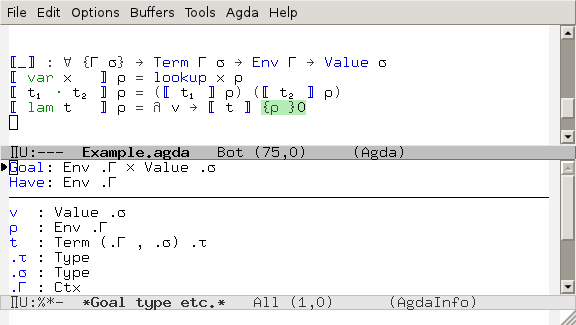
\includegraphics[scale=1.2]{emacs.png}
          \end{minipage}
        \end{block}

      \end{column}
      \begin{column}{.45\textwidth-1ex}%
        \begin{block}{Formalization}
          Coq, Agda
        \end{block}

      \end{column}
    \end{columns}

    \begin{block}{Hott}
      lsdkjflsdk
    \end{block}

  \end{block}
\end{frame}

\end{document}


%%% Local Variables: 
%%% mode: latex
%%% TeX-master: t
%%% End: 
